\begin{frame}{}
    \LARGE Advanced Diffusion Models: \textbf{Latent Space Diffusion (Stable Diffusion)}
\end{frame}

\begin{frame}[allowframebreaks]{Latent Diffusion Models}

    \begin{itemize}
        \item Pixel-space diffusion models are computationally expensive.
        \item Can we learn a compressed latent space, similar to approaches in autoregressive models (e.g., VQGAN)?
        \item Solution: Train a Variational Autoencoder (VAE) with a very low weighting on the KL divergence loss (e.g., $10^{-6}$) to obtain a compact latent representation.
    \end{itemize}

    \begin{figure}
        \centering
        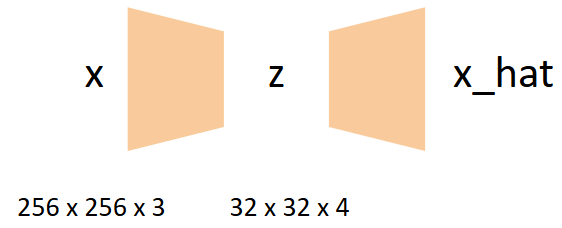
\includegraphics[width=0.5\linewidth,height=0.4\textheight,keepaspectratio]{images/adv-img-gen/slide_96_1_img.png}
        \caption*{Rombach, Robin, et al. "High-resolution image synthesis with latent diffusion models." Proceedings of the IEEE/CVF conference on computer vision and pattern recognition. 2022.}
    \end{figure}

    \framebreak

    \textbf{Key Concepts}
    \begin{itemize}
        \item \textbf{Latent Diffusion Models (LDMs):} Operate in a compressed latent space for efficiency.
        \item \textbf{Diffusion Process:} Gradually adds noise to data, then learns to reverse this process.
        \item \textbf{Text Conditioning:} Uses CLIP text encoders to guide image generation from prompts.
    \end{itemize}

    \framebreak

    \begin{figure}
        \centering
        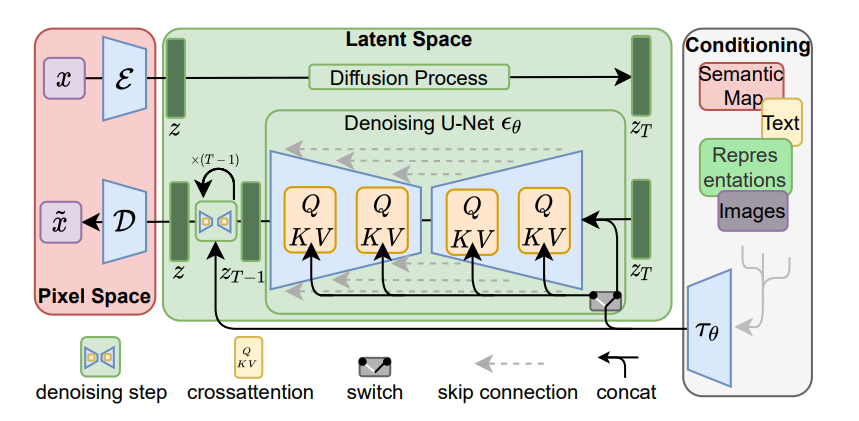
\includegraphics[width=1.05\linewidth,height=0.95\textheight,keepaspectratio]{images/adv-img-gen/slide_97_1_img.png}
    \end{figure}

    \framebreak

    \textbf{Architecture Overview}
    \begin{itemize}
        \item \textbf{Encoder:} Maps images to latent space.
        \item \textbf{UNet:} Core denoising network operating in latent space.
        \item \textbf{Decoder:} Reconstructs images from latent representations.
        \item \textbf{Text Encoder:} CLIP-based, encodes prompts for conditioning.
    \end{itemize}

    \framebreak

    Speed - Quality Trade-off

    \begin{columns}
        \column{0.6\textwidth}
            \begin{figure}
                \centering
                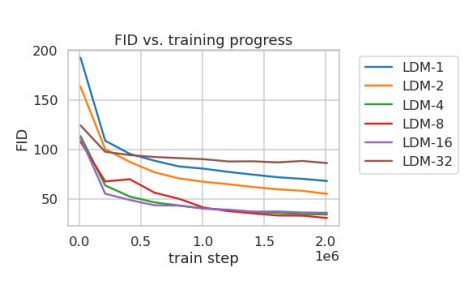
\includegraphics[width=1.05\linewidth,height=\textheight,keepaspectratio]{images/adv-img-gen/slide_98_1_img.png}
            \end{figure}
        \column{0.5\textwidth}
            \begin{figure}
                \centering
                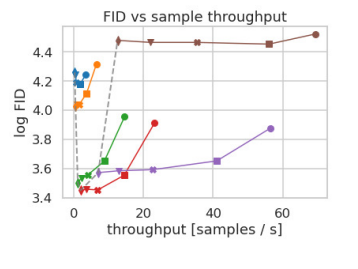
\includegraphics[width=\linewidth,height=\textheight,keepaspectratio]{images/adv-img-gen/slide_98_2_img.png}
            \end{figure}
    \end{columns}   
    
\end{frame}

\begin{frame}[allowframebreaks]{Stable Diffusion}
    \textbf{What is Stable Diffusion?}
    \begin{itemize}
        \item A state-of-the-art text-to-image generative model.
        \item Developed by Stability AI and collaborators (2022).
        \item Open-source, enabling wide adoption and customization.
    \end{itemize}

    \framebreak

    \begin{itemize}
        \item VAE that downsamples images by 8x spatially (e.g., $256 \rightarrow 32$, $512 \rightarrow 64$).
        \item UNet architecture with self-attention layers.
        \item Text conditioning via cross-attention on text features.
        \item Text features extracted using a CLIP text encoder.
    \end{itemize}
    \vspace{1em}
    \begin{figure}
        \centering
        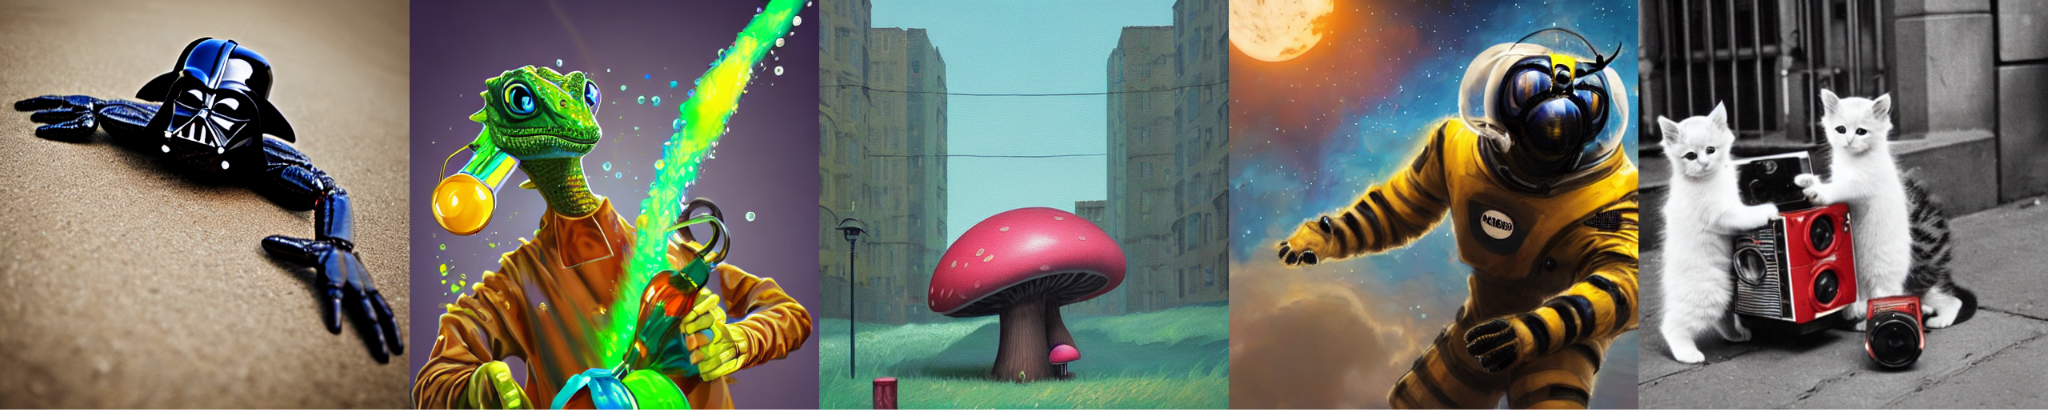
\includegraphics[width=1.06\linewidth,height=\textheight,keepaspectratio]{images/adv-img-gen/slide_99_1_img.png}
    \end{figure}

    \framebreak

    \textbf{Advantages}
    \begin{itemize}
        \item High-quality, diverse image generation.
        \item Efficient training and inference due to latent space operations.
        \item Open-source and extensible for research and applications.
    \end{itemize}

    \textbf{Applications}
    \begin{itemize}
        \item Art and creative design.
        \item Data augmentation.
        \item Prototyping and visualization.
    \end{itemize}

    \framebreak

    \textbf{Recent Advances and Ecosystem}
    \begin{itemize}
        \item \textbf{Stable Diffusion XL (SDXL):} Improved fidelity and prompt adherence.
        \item \textbf{ControlNet:} Fine-grained control over generation (e.g., pose, edges).
        \item \textbf{Community Models:} Custom fine-tuned models for specific styles/domains.
    \end{itemize}

\end{frame}

\begin{frame}[allowframebreaks]{Stable Video Diffusion}
    \begin{itemize}
        \item Initialize from Stable Diffusion.
        \item Add temporal layers (e.g., 1D Conv, temporal attention).
        \item Finetune on video data.
        \item Data pipeline:
        \begin{itemize}
            \item Scrape \textbf{unlabeled} videos from the internet.
            \item Use image and video captioners to generate synthetic text labels.
            \item Apply aggressive data filtering using several heuristics (CLIP score, optical flow score, aesthetic scores, OCR, etc.).
        \end{itemize}
    \end{itemize}
    
    \framebreak

    \begin{figure}
        \centering
        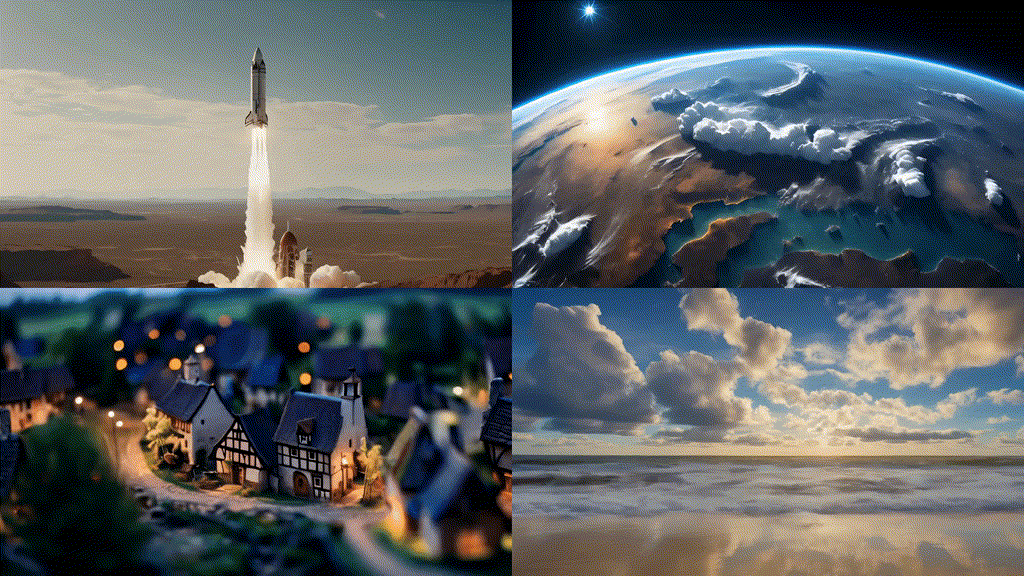
\includegraphics[width=1.06\linewidth,height=\textheight,keepaspectratio]{images/adv-img-gen/slide_101_1_img.png}
        \caption*{\href{https://drive.google.com/file/d/19XVG5MpxMRXP1hwHETkP_prlbHOcuTSj/view?usp=sharing}{Link: GIFF}}
    \end{figure}

    % \textbf{References}
    % \begin{itemize}
    %     \item Rombach et al., "High-Resolution Image Synthesis with Latent Diffusion Models", CVPR 2022.
    %     \item Official Stable Diffusion GitHub: \url{https://github.com/CompVis/stable-diffusion}
    % \end{itemize}
\end{frame}